\documentclass{cslthse-msc}
\usepackage[utf8]{inputenc}
\usepackage[english]{babel}
\usepackage{amsmath}
\usepackage{amsfonts}
\usepackage{amssymb}
\usepackage{amsthm}
%\usepackage{makeidx}
\usepackage{graphicx}
\usepackage[titletoc, header, page]{appendix}
\usepackage{multirow}% http://ctan.org/pkg/multirow
\usepackage{hhline}% http://ctan.org/pkg/hhline
\usepackage{hyperref}
\usepackage{pdfpages}
\usepackage{rotating}
\usepackage{enumitem}
\usepackage{subfig}
\usepackage{float}
\usepackage{listings}
\usepackage{epstopdf}
\usepackage{comment}
\usepackage{hyperref}
%% listings-modelica.cfg
%% Copyright 2014 Martin Sjoelund, Dietmar Winkler
%
% This work may be distributed and/or modified under the
% conditions of the LaTeX Project Public License, either version 1.3
% of this license or (at your option) any later version.
% The latest version of this license is in
%   http://www.latex-project.org/lppl.txt
% and version 1.3 or later is part of all distributions of LaTeX
% version 2005/12/01 or later.
%
% This work has the LPPL maintenance status `maintained'.
%
% The Current Maintainer of this work is Dietmar Winkler
%
% Code repository https://github.com/modelica-tools/listings-modelica
%
% This work consists of the file listings-modelica.cfg

\lstdefinelanguage{modelica}
{
  morekeywords=[1]{
    algorithm,and,annotation,as,assert,block,break,case,class,connect,connector,
    constant,constrainedby,der,discrete,each,else,elseif,elsewhen,encapsulated,
    end,enumeration,equality,equation,expandable,extends,external,failure,final,
    flow,for,function,guard,if,import,in,initial,inner,input,List,local,loop,
    match,matchcontinue,model,not,operator,Option,or,outer,output,package,parameter,
    partial,protected,public,record,redeclare,replaceable,return,stream,
    subtypeof,then,Tuple,type,uniontype,when,while},
  morekeywords=[2]{true, false},
  % Do not make true,false keywords because fn(true,x, false ) shows up as fn(true,x, *false*)
  sensitive=true,
  comment=[l]//,
  morecomment=[s]{/*}{*/},
  alsodigit={.,-},
  morestring=[b]',
  morestring=[b]",
}[keywords,comments,strings]

\definecolor{keywordcolor1}{rgb}{0,0,.4}
\definecolor{keywordcolor2}{rgb}{.90,0,0}
\definecolor{stringcolor}{rgb}{0.133,0.545,0.133}
% \definecolor{listingbgcolor}{rgb}{0.95,0.95,0.95}

\lstset{
  breaklines=true,
  language=modelica,
  basicstyle=\ttfamily,
  keywordstyle=[1]\color{keywordcolor1}\bfseries,
  keywordstyle=[2]\color{keywordcolor2},
  stringstyle=\color{stringcolor},
%  backgroundcolor=\color{listingbgcolor},
  framexleftmargin=5pt,
  xleftmargin=5pt,
  xrightmargin=5pt,
  showstringspaces=false
}

\newcommand{\code}[1]{\lstinline|#1|}
\newcommand{\modelica}[1]{\lstinline[language=modelica]|#1|}

\usepackage{makecell}
\usepackage[style=numeric]{biblatex}
\addbibresource{thebib.bib}% 
%\geometry{showframe}
\DefineBibliographyStrings{english}{%
  bibliography = {References},
}
\author{
	Erik Hedblom \\
	{\normalsize \href{mailto:hedblom.e@gmail.com}{\texttt{hedblom.e@gmail.com}}}
	\and
	Kasper Rundquist \\
	{\normalsize \href{mailto:kasper.rundquist@gmail.com}{\texttt{kasper.rundquist@gmail.com}}}
}

\title{Safe test selection for Modelica using static analysis}
%\subtitle{A {\LaTeX} class}
\company{Modelon AB}
\supervisors{Johan Ylikiiskilä, \href{mailto:johan.ylikiiskila@modelon.com}{\texttt{johan.ylikiiskila@modelon.com}}}{Jonatan Kämpe, \href{mailto:jonathan.kampe@modelon.com}{\texttt{jonathan.kampe@modelon.com}}}{Niklas Fors, \href{mailto:niklas.fors@cs.lth.se}{\texttt{niklas.fors@cs.lth.se}}}%\supervisor{Niklas Fors, \href{mailto:niklas.fors@cs.lth.se}{\texttt{niklas.fors@cs.lth.se}}}
\examiner{Görel Hedin, \href{mailto:gorel.hedin@cs.lth.se}{\texttt{gorel.hedin@cs.lth.se}}}

\date{\today}
%\date{January 16, 2015}

\acknowledgements{
We would like to thank Johan Ylikiiskilä at Modelon, who proposed the subject of this master thesis and has introduced us to Model Testing Toolkit.

Further we would like to thank Jonathan Kämpe and Jesper Mattsson at Modelon for helping us understand the JModelica.org compiler and validate our dependency analysis.

We would also like to thank our supervisor at LTH, Niklas Fors for all feedback during our work on the report.

%%If you want to thank people, do it here, on a separate right-hand page. Both the U.S. \textit{acknowledgments} and the British \textit{acknowledgements} spellings are acceptable.
}

\theabstract{
During software development, testing of software can be very time consuming. We have developed a safe regression test selection technique using static analysis, for the modeling language Modelica. When a user changes a Modelica model, our technique will exclude tests that are guaranteed not to be affected by the change. Since Modelica tests usually has relatively long running times there is much time to save. As far as we know test selection has previously not been attempted for Modelica. To perform the test selection we have implemented a dependency analysis in an existing Modelica compiler. We have evaluated our technique and tried to assess how much time that can be saved. When we look at the commit history of the Modelica Standard Library and compare running all tests with only running the tests selected by our test selection, the time saved for running the selected tests is 56\% of the time it takes to run all tests.

%%Your abstract should capture the whole thesis with focus on the problem and solution in 150 words. Avoid acronyms, footnotes, and references in the abstract if possible.

}

\keywords{Test Selection, Modelica, Regression testing, JModelica.org}
\divisionoflabor{
Throughout this thesis project we, Erik and Kasper, have not had a clear devision of labor. We have been seated next to each other and naturally this has allowed to discuss and participate in all aspects of the project together. 
}

%% Only used to display font sizes
\makeatletter
\newcommand\thefontsize[1]{{#1 \f@size pt\par}}
\makeatother
%%%%%%%%%%


\begin{document}
\makefrontmatter
\chapter[Introduction]{Introduction}

\section{Motivation}
Software tests are used to verify that software works as intended.
During software development, when a change is integrated into a project all previous testing have to be rerun to ensure no regression has occurred \cite{DBLP:conf/sigsoft/LegunsenHSLZM16, haider2016safe}. This is know as \emph{regression testing}. Test suites usually accumulates over time and regression testing can therefore be very time consuming. Depending on the change some or most of the tests may be unrelated to the change and therefore unnecessary to run. By excluding unrelated tests significant time savings could be achieved. Choosing which tests to run is called \emph{test selection}. When the test selection is done for regression tests it is known as \emph{regression test selection} (RTS).

%TODO: Okay to have ha Modelica section under Motivation? Or we need a specific Modelica section with its own heading?
%TODO: Good examples of areas where Modelica is used?
\emph{Modelica} is an object oriented modeling language used for simulations in various areas, for example simulations of electrical components, engines and air conditioners. Usually Modelica tests has long execution times. To our knowledge test selection has not been previously developed for Modelica.



\section{Goal}
%TODO: Correct to say that: we are going to implement in the JModelica.org compiler when we acctually do it in OCT? Niklas thought that we should write about JModelica in the introduction
%TODO: Correct to say that: the goal is to give some Modelica models to the compiler, when it origanally was files?
The aim of this project is to reduce testing times for Modelica projects without loss of quality. This will be done by developing and implementing a safe RTS method with static analysis, a method to exclude tests in a test suite unaffected by a specific change \cite{DBLP:conf/pppj/OqvistHM16}. Regression testing can then be performed with a reduced test suite without compromising testing quality. To know which tests can be safely excluded we need to know if there is dependencies between different parts of Modelica code. To solve this we are going to implement a solution in the JModelica.org compiler. The goal is to be able to give some Modelica models to the compiler and get a dependency graph of Modelica classes.

\section{Results}
We have succeeded in significantly decreasing the time for testing by using test selection for Modelica. In chapter 5 we evaluate our solution, we try to assess how much time can be saved with our RTS method and the precision of the method. We look at the commit history for some Modelica libraries to see how much time would have been saved if our RTS method had been used instead of running all tests for each commit. However we have not formally proved that the method we have developed is safe, we discuss this further in chapter 6.

\chapter[Background]{Background}
In this chapter we will explain concepts and give some background important to understanding the rest of the report. We will give a short explanation of test selection, the Modelica language and a summary of how the JModelica.org compiler works.

\section{Test Selection}
A safe Regression Test Selection (RTS) method will select at least all tests that produce a new result after a specific change \cite{DBLP:conf/pppj/OqvistHM16}. A safe RTS method is therefore equivalent to running all tests, in the aspect of finding errors. For a RTS method to be useful the RTS algorithm should run in less time than it takes to run the excluded tests. This is not necessary for each run, but on average the overhead needs to be less than the time it takes to run the excluded tests.

To measure how good the test selection is, the precision of the test selection can be used \cite{DBLP:conf/sigsoft/LegunsenHSLZM16}. If fewer redundant tests are selected, the test selection has higher precision. There is a trade-off between the precision of the test selection and the overhead. To get higher precision, a more complex algorithm may be needed.

\section{Modelica}
Modelica is a declarative, object oriented modeling language where models are described by equations \cite{modelicamodelica}. It is used to perform high performance simulations. This section will introduce the parts of Modelica that is important for this project. In Figure \ref{fig:bouncingBallCode} is a simple Modelica example to illustrate the language. It shows a model of a bouncing ball and in Figure \ref{fig:bouncingBallSimulation} is the simulation result of the bouncing ball model.

\begin{figure}[!htbp]
    \centering
    \lstinputlisting[language=modelica]{Modelica/BouncingBall.mo}
    \caption{A Modelica model of a bouncing ball. This example is inspired by \textit{Implementation of a Modelica compiler using JastAdd attribute grammars} \cite{aakesson2010implementation} and \textit{Modelica by example} \cite{tillermodelica}.}
    \label{fig:bouncingBallCode}
\end{figure}

\begin{figure}[!htbp]
    \centering
    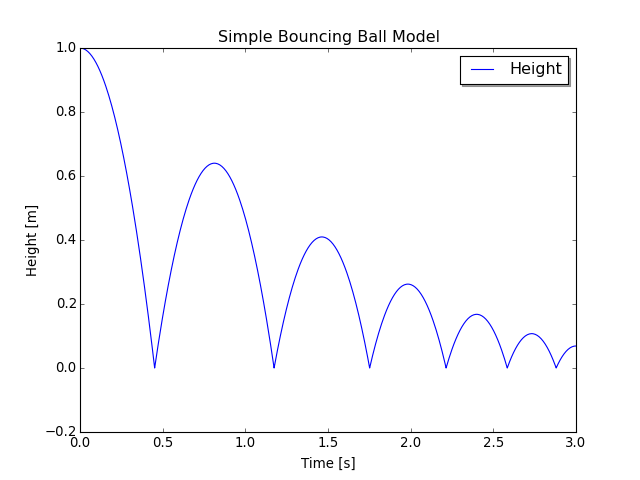
\includegraphics[width=1.0\textwidth]{Pictures/BB1.png}
    \caption{The simulation result of the model in Figure \ref{fig:bouncingBallCode}. This graph is retrieved from \textit{Modelica by example} \cite{tillermodelica}}
    \label{fig:bouncingBallSimulation}
\end{figure}

Modelica uses dot notation to access something inside an object \cite{modelicamodelica}. Consider the code snippet in Figure \ref{fig:modelicaExample}, the model \texttt{M} can be accessed through \texttt{P1.P2.M}. We will call this an \emph{access}. Depending on from which scope \texttt{M} is being accessed, the access could also be \texttt{P2.M} or just \texttt{M}. An access using dot notation is basically a list of accesses and we will call all the accesses the \emph{path}. For instance, the path of model \texttt{M} is \texttt{P1.P2.M}. We will also denote a path as a \emph{fully qualified name}, if the first part of it is referencing the top package. In this case the fully qualified name for \texttt{M} is \texttt{P1.P2.M}.

\begin{figure}[!htbp]
    \centering
    \subfloat{{\includegraphics[scale=0.8]{dotGenerated/ModelicaExample.eps}}}
    \qquad
    \subfloat{\raisebox{3.2 cm}{\lstinputlisting[language=modelica]{Modelica/ModelicaExample.mo}}}
    \caption{An example of Modelica structure, where the boxes represents the Modelica classes in the Modelica code to the right.}
    \label{fig:modelicaExample}
\end{figure}

It is not apparent from an access what it is trying to access, it could be a package, model, function or a component. Due to this we will simplify the terminology by grouping models, packages and function together and just call them classes. Components are instantiations of classes and will be handled separately.

\subsection{Name lookup}
In this section we will give an example of a name lookup in the Modelica compiler. For an exhaustive description of the Modelica name lookup, see the Modelica specification \cite{modelicamodelica}. In order to find a match for a name, the Modelica compiler starts by looking at the first name in the path \cite{modelicamodelica, tillermodelica}. In Figure \ref{fig:nameLookup}, when \texttt{P1.P3.M.x} is defined it is initialized to the value the constant \texttt{P1.P2.k} has. To find the constant \texttt{k} through the path \texttt{P2.k}, the Modelica compiler starts by trying to find a match for the first name, \texttt{P2}, in the path. The Modelica compiler first checks if there is a definition of \texttt{P2} in the class \texttt{M}, where it is used. There is no definition of of \texttt{P2} in class \texttt{M}, so the Modelica compiler continues by looking for a definition in the enclosing class \texttt{P3}. There is still no definition of \texttt{P2}, in the next step the Modelica compiler looks for a definition in the enclosing class of \texttt{P3}, package \texttt{P1}. In package \texttt{P1} a definition of the name \texttt{P2} is found. Then the Modelica compiler looks for a definition of the name \texttt{k} in the class \texttt{P2}, and finds a definition of \texttt{P2.k}.

\begin{figure}[!htbp]
    \centering
    \lstinputlisting[language=modelica]{Modelica/NameLookup.mo}
    \caption{An example to illustrate the name lookup in the Modelica compiler.}
    \label{fig:nameLookup}
\end{figure}

\subsection{Import}
In Modelica imports can be used to access objects without using the fully qualified name each time, an import creates an alias \cite{tillermodelica}. Imports are also used to affect the name lookup and avoid name shadowing. To find an imported object the Modelica compiler looks for a match for the name in root packages, so the fully qualified name needs to be used in an import statement. In the import below \texttt{HydralicConductance} will be mapped to the fully qualified name \texttt{Modelica.Fluid.Types.HydralicConductance}.

\lstinputlisting[language=modelica]{Modelica/import.mo}

Modelica offers the option to rename an import. Here an alias will be created where the name \texttt{Conductance} is mapped to the fully qualified name \\\texttt{Modelica.Fluid.Types.HydralicConductance}.

\lstinputlisting[language=modelica]{Modelica/renamedImport.mo}

Modelica allows the use of wildcard imports. When using wildcard imports it is not possible to rename the import. This wildcard import will create an alias for every definition in \texttt{Modelica.Fluid}.

\lstinputlisting[language=modelica]{Modelica/wildcardImport.mo}

\section{JModelica.org}
JModelica.org is an open source compiler developed and maintained by the company Modelon. Optimica Compiler Toolkit (OCT) is the commercial version of JModelica.org. Our solution will be developed in OCT but will not use any OCT specific functionality. 

The compilation of Modelica code in JModelica.org is done in several steps, see Figure \ref{fig:compilerSteps} \cite{aakesson2010implementation}. In the first step, name and type analysis of the source code is done, identifiers are bound to declarations etc. An AST (Abstract Syntax Tree) is built in form of a source tree.

In Figure \ref{fig:bouncingBallInstance} when the instance of \texttt{BouncingBall}, \texttt{Ball} in Figure \ref{fig:bouncingBallCode} is created, a modification is used to set the gravity to a different value than the original. The flattening of Modelica code is complicated because of modifications that are used in Modelica. To simplify this and  prepare for the flattening, in step two a new AST in form of a instance tree is generated from the source tree. Each node in the instance tree has a reference to the corresponding declaration in the source tree. The root is the model chosen by the user to be flattened. The instance tree consists of instances of all classes with the possibly given modifications at the point in the Modelica source code where the instance is created. Therefore the instance tree requires a lot more memory than the source tree and is slower to traverse. This is the reason we have chosen to implement our solution in the source tree. 

In the third step the Modelica code is flattened. In this step class, component and inheritance structures are removed. This results in a model that only has a set of equations and a set of variables. Since an instance tree is created in the previous step, it is easy to traverse the instance tree and collect all variables and equations to create the flat tree.

In the fourth step the equations are sorted and optimized.

In the last step C-code is generated.

\begin{figure}[!htbp]
    \centering
    {\includegraphics[scale=0.5]{dotGenerated/CompilerSteps.eps}}
    \caption{The compilation steps in the JModelica.org compiler}
    \label{fig:compilerSteps}
\end{figure}

\begin{figure}[!htbp]
    \centering
    \lstinputlisting[language=modelica]{Modelica/BouncingBallInstance.mo}
    \caption{Instance of the bouncing ball in Figure \ref{fig:bouncingBallCode} with modification. This example is inspired by \textit{Implementation of a Modelica compiler using JastAdd attribute grammars} \cite{aakesson2010implementation}.}
    \label{fig:bouncingBallInstance}
\end{figure}

\section{Model Testing Toolkit}
Model testing Toolkit (MTT) is a toolbox developed by Modelon to handle testing of Modelica projects \cite{modelon.comMTT}. It has both a command line and a graphical interface and we will add functionality and options to both to support test selection. Furthermore, it also provides integration with third-party tools. This means that compilers other than JModleica.org could be used together with MTT.


\chapter[Dependency analysis]{Dependency analysis}
To implement the RTS (Regression Test Selection) for Modelica we build a dependency graph between Modelica classes in the compilation phase. To build the dependency graph we have constructed a set of rules to determine what creates dependencies. We have chosen to work with the source tree representation of Modelica programs in the JModelica.org compiler. The source tree is a relative light weight representation of a Modelica program and have limited name lookup capabilities but provides significant performance benefits. The rules have therefore been adjusted to work with the name lookup in the source tree. When the lookup of an access fails in the source tree we say the access is not resolvable. This means that a valid access can fail to resolve, in the source tree. First we introduce the rules and then we will go on and explain and motivate each one. Then we will conclude this chapter by discussing the limitations and improvements of the dependency analysis.

\paragraph{Dependency Rules}\mbox{}\\
To build the dependency graph we use the following rules:
\begin{enumerate}
\item A class depends on all resolvable accesses within it.
\item A class depends on its enclosing class. 
\item All resolvable accesses in the path of an access yields dependencies.
\item A class depends on all classes enclosed by the accessed class. If the access is not resolvable, the last resolvable access in the path will be used instead.
\item Exception to Rule 4: Rule 4 is not applicable to import statements. An import should not add dependencies to classes not imported but the import.
\end{enumerate}


\begin{figure}[!htbp]
    \centering
    \subfloat{{\includegraphics[scale=0.8]{dotGenerated/Parent.eps}}}
    \qquad
    \subfloat{\raisebox{3.2 cm}{\lstinputlisting[language=modelica]{Modelica/Parent.mo}}}
    \caption{To the right an example of Modelica code showing why Rule 2 is needed, and to the left the corresponding dependency graph.}
    \label{fig:parentGraph}
\end{figure}
The first rule is perhaps the most intuitive, if a class accesses another class there is also a dependency to that class. However, due to the limitations in the source tree in JModelica.org not all accesses in a class can be followed and therefor not all dependencies from this rule can be created. We will later see how Rule 4 compensates for this. 

The next rule, Rule 2, will create a dependency from a class to its enclosing class. An example can be found in Figure \ref{fig:parentGraph}. In the example there is a constant \texttt{k} defined in package \texttt{P}. If another constant with the same name were to be added in in model \texttt{M1} the reference to \texttt{k} in \texttt{M2} will change to refer to the new constant and shadow the \texttt{k} in \texttt{P}. Therefore we need a dependency from \texttt{M2} to \texttt{M1} to handle name shadowing.

In Figure \ref{fig:parentGraph} we also expect Rule 1 to create a dependency from \texttt{M2} to \texttt{P} due to \texttt{k} being located in \texttt{P}. However, the access \texttt{k} cannot be resolved by the JModelica.org compiler in the source tree and we will miss the dependency to \texttt{P}. In this case we can see that Rule 2 can compensate by adding an indirect dependency from \texttt{M2} to \texttt{P}. 
If the constant \texttt{k} in package \texttt{P} is changed it will affect model \texttt{M2}. Therefore we need a dependency from \texttt{M2} to \texttt{P}. With Rule number 2 we get dependencies from \texttt{M2} to \texttt{M1} and from \texttt{M1} to \texttt{P}. So we have an indirect dependency from \texttt{M2} to \texttt{P}.

\begin{figure}[!htbp]
    \centering
    \subfloat{{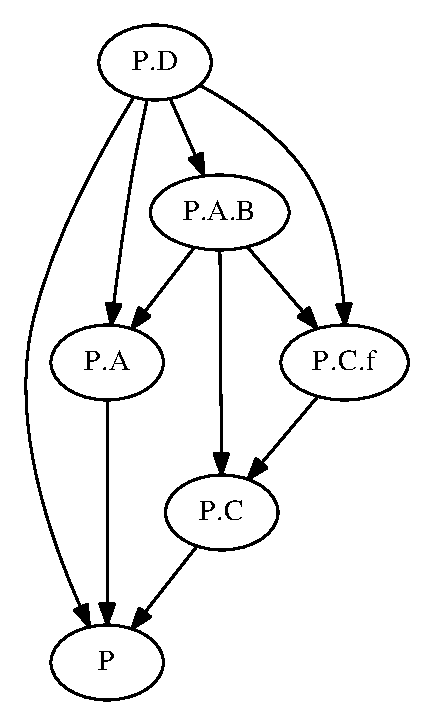
\includegraphics[scale=0.8]{dotGenerated/DotAccess.eps}}}
    \qquad
    \subfloat{\raisebox{9.5 cm}{
        \begin{minipage}[t]{.5\textwidth}
        \centering
        \lstinputlisting[language=modelica]{Modelica/DotAccess.mo}
        \end{minipage}}}
    \caption{Dependency graph to the left, of the Modelica classes to the right. This is an example of why we need Rule 3.}
    \label{fig:dotAccess}
\end{figure}

In Figure \ref{fig:dotAccess}, we want dependencies from model \texttt{M} to all parts of the access to \texttt{f}. This means that in addition to a dependency to \texttt{f}, a dependency to \texttt{P3} is also required. If package \texttt{P3} is removed it will cause a compilation error when model \texttt{M} is compiled. Also, if \texttt{f} is shadowed in \texttt{P3} the behavior of model \texttt{M} will change. This is caught by Rule 3, that creates dependencies from \texttt{M} to \texttt{f} and \texttt{P3}.


\begin{figure}[!htbp]
    \centering
    \subfloat{{\includegraphics[scale=0.8]{dotGenerated/Component.eps}}}
    \qquad
    \subfloat{\raisebox{4.7 cm}{\lstinputlisting[language=modelica]{Modelica/Component.mo}}}
    \caption{To the right Modelica code with an access through a component, \texttt{m.M3.f(1)}, this is the reason Rule 4 is needed. To the left is the dependency graph.}
    \label{fig:component}
\end{figure}

Rule 4 is needed to handle the case in Figure \ref{fig:component}. Ideally the access \texttt{m.M3.f} would create dependencies to \texttt{M2}, \texttt{M3} and \texttt{f}. Because \texttt{m} is a component and the analysis is done in the source tree, \texttt{m.M3.f} cannot be resolved and no dependencies can be created. Instead Rule 4 is used to create dependencies to everything defined in \texttt{M2} when \texttt{m} is declared.

\begin{figure}[!htbp]
    \centering
    \subfloat{{\includegraphics[scale=0.8]{dotGenerated/Rule5.eps}}}
    \qquad
    \subfloat{\raisebox{4.0 cm}{\lstinputlisting[language=modelica]{Modelica/Rule5.mo}}}
    \caption{Example of rule 5 improving the dependency graph. The dashed edges are removed by Rule 5.}
    \label{fig:rule5}
\end{figure}

Rule 5 is an exception to Rule 4, added to improve the precision of the test selection. Imports are specific and it is enough to add dependencies to what is actually imported. It is not uncommon to import packages located high up in the library structure. Without this exception, unnecessary dependencies would be added to all or large part of the library. For example in Modelica's standard library there are several imports of Modelica, which is the top level package. Such imports would create dependencies to every single class in the library. (Such imports may seem unnecessary, but they can be used to affect the name lookup if there exists classes with the same name in the library). An example of this is shown in Figure \ref{fig:rule5}.

\section{Discussion}
The lookup limitation in the source tree of JModelica.org have had significant impact on the dependency analysis. It would be interesting to explore the differences compared to a dependency analysis only considering the Modelica standard and not limited by the source tree in JModelica.org. We have looked at the option of improving the lookup in the source tree in JModelica.org. However, that seems unfeasible within our time frame and furthermore, the functionality is already available in the instance tree.

It would be interesting to explore the option of performing the dependency analysis in the instance tree. The main problem with this is the memory requirements, to instantiate all classes in one or more libraries would likely require to much memory. It might be possible to work around this by building the dependency graph incrementally. There is also currently some work into throwing away parts of the instance tree to save memory so that might also be a viable option in the future. The running time such solutions would probably be significantly higher and would have to be compensated by the precision gain in the dependency graph. 

Another concern with a more precise dependency analysis is differences between compilers, since the solution is used through MTT and MTT might not use JModelica.org when compiling and running tests. For example, error checking might differ between compilers causing compilation error for a test using one compiler but not for another.

A more precise dependency analysis would probably be more complicated. Consider the example in Figure \ref{fig:contrainedBy}. A more precise dependency analysis would have to find out that the function call \texttt{m.f(10)} refers to \texttt{P5.f} but also depend on at least \texttt{P4} and \texttt{P3} due to the constraints on \texttt{f}. However, \texttt{f} might also depend on \texttt{P1} and \texttt{P2} if the compiler error check the constraints. 

\begin{figure}[htbp]
    \centering
    \raisebox{4.0 cm}{\lstinputlisting[language=modelica]{Modelica/ConstrainedBy.mo}}
    \caption{An example illustrating some complex dependencies}
    \label{fig:contrainedBy}
\end{figure}


\chapter[Implementation]{Implementation}
In this chapter we will describe how we have implemented the test selection in JModelica.org. The solution is implemented both in Optimica Compiler Toolkit (OCT) and in Model Testing Toolkit (MTT). OCT will produce the dependency graph and MTT will interact with the user and run the reduced test suit.

\section{Model Testing Toolkit}

MTT will process the data from the user, either from the command line interface (CLI) or from the graphical user interface (GUI). We have added an option to the CLI so that the user can specify that test selection should be used and which models or files have changed. In the GUI we have added a menu option to specify which models have changed, this is shown in Figure \ref{fig:MTTrun}. In the GUI multiple models can be selected.

\begin{figure}[!hbtp]
    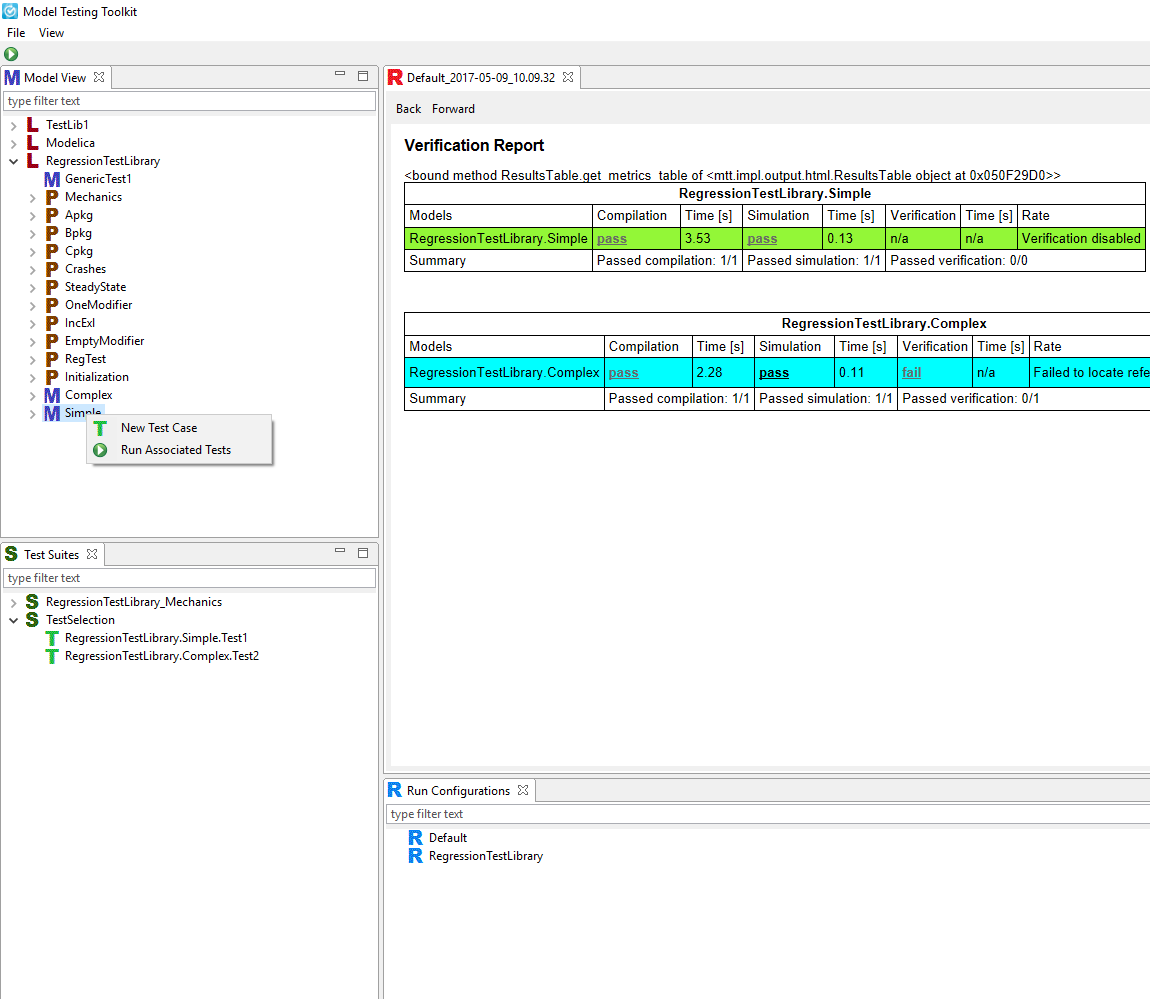
\includegraphics[width=1.0\textwidth]{Pictures/MTT_Capture.png}
    \caption{A screen shot of the MTT GUI. In the Model View pane the when right clicking on a Model there is an option to run all associated tests.}
    \label{fig:MTTrun}
\end{figure}

MTT will then send all modified files or models to OCT and ask for all affected models. Then tests, testing one of the affected models, will be selected and run.

\subsection{Change detection}
There is no automatic change detection, instead the user manually have to specify which models or files should be considered changed. Automatic change detection could be implemented using a version control system such as Git or SVN. A continuous integration server could look at the commit history to determine what is changed. For a user using MTT \texttt{git status} could be used. Another option is to look at the file timestamps to determine what is changed.

\section{Dependency analysis}
We have previously described how the dependency analysis should be performed. In this section we will look at some of the aspects not handled by the rules presented in Chapter 3.

\subsection{Scope}
To speed up the dependency analysis we ask the user to specify which libraries should be search for dependencies. For example, the standard library is automatically included in projects but users will rarely make changes to or test it. Hence, searching for dependencies to and in the standard library will usually be unnecessary. There might also be other dependencies in a project that are considered stable and unnecessary to analyze. In MTT this is handled by automatically search in all libraries in the Model View pane, in the upper left part of Figure \ref{fig:MTTrun}.

Furthermore, our implementation also excludes Modelica built-ins. Built-ins such as \texttt{Real} should never change, and if they do, it means the compiler has changed. If the compiler has changed all test will have to be rerun anyway.

\subsection{Inverted dependency graph}
The dependency graph produced in Chapter 3 shows the dependencies from the compilers perspective. To find out which models are affected by a change the graph has to be inverted. Consider the left graph in Figure \ref{fig:invertedGraph}, if the class \texttt{C2} is changed the graph has to be searched backwards to find out that the test \texttt{T2} should be selected. This is implemented by inverting the dependency graph, resulting in the right graph in Figure \ref{fig:invertedGraph}.

\begin{figure}[!htbp]
    \centering
    \subfloat{{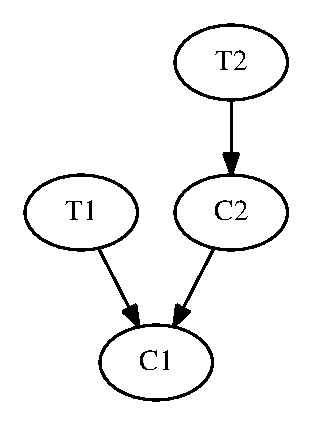
\includegraphics[scale=0.8]{dotGenerated/GraphExample.eps}}}
    \qquad
    \subfloat{{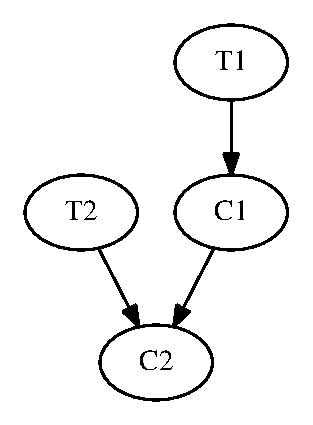
\includegraphics[scale=0.8]{dotGenerated/InvertedGraphExample.eps}}}
    \caption{To the left is a dependency graph and to the right is the corresponding inverted dependency graph. T1 and T2 are test cases and C1 and C2 are Modelica classes.}
    \label{fig:invertedGraph}
\end{figure}

\subsection{External functions}
The Modelica language allows use of external functions that are not defined in a Modelica file. The external functions are often defined in a C-files\cite{modelicamodelica}. In our dependency analysis we do not analyze the dependencies in external files. To handle this, and keep the test selection safe, if a non Modelica file is changed we assume that every Modelica class that depend on externals are affected.


\chapter[Evaluation]{Evaluation}
In this chapter we are evaluating the performance of our dependency analysis and test selection. We have performed measurements for HXL (the Heat Exchanger Library developed by Modelon \footnote{\url{http://www.modelon.com/products/modelica-libraries/heat-exchanger-library/}}) and MSL (Modelica Standard Library). To assess how much time our test selection can save, we have run the tests for each library several times, 31 times for MSL and 7 for HXL, to get the average time it takes to run each test. This was done using a Intel\textregistered Core \texttrademark i5-4300M. The test times will be used to simulate a test selection without having to run the tests. Some tests have very long running times, therefore we limited tests to ten minutes. Test taking longer will timeout and their running time is set to ten minutes.

First we preformed test selection for each Modelica file in two libraries, MSL and HXL, and assumed only one file changed. The total test suite execution time was 2h 26m 35s for MSL and 3h 1m 51s for HXL. In Figure \ref{fig:hxlonefile} and \ref{fig:mslonefile} the result for all files in HXL and MSL relative the total execution time for the complete test suite is shown. Neither of the graphs include the execution time of the test selection algorithm and therefore the time savings are not completely accurate. However, in both cases the the test selection time corresponds to a fraction of a percent on the y-axis. Figure \ref{fig:hxlonemodel} and \ref{fig:mslonemodel} are similar to Figure \ref{fig:hxlonefile} and \ref{fig:mslonefile} but the selection is performed with a finer granularity, using models instead of files. 

\begin{figure}[!htbp]
    \centering
    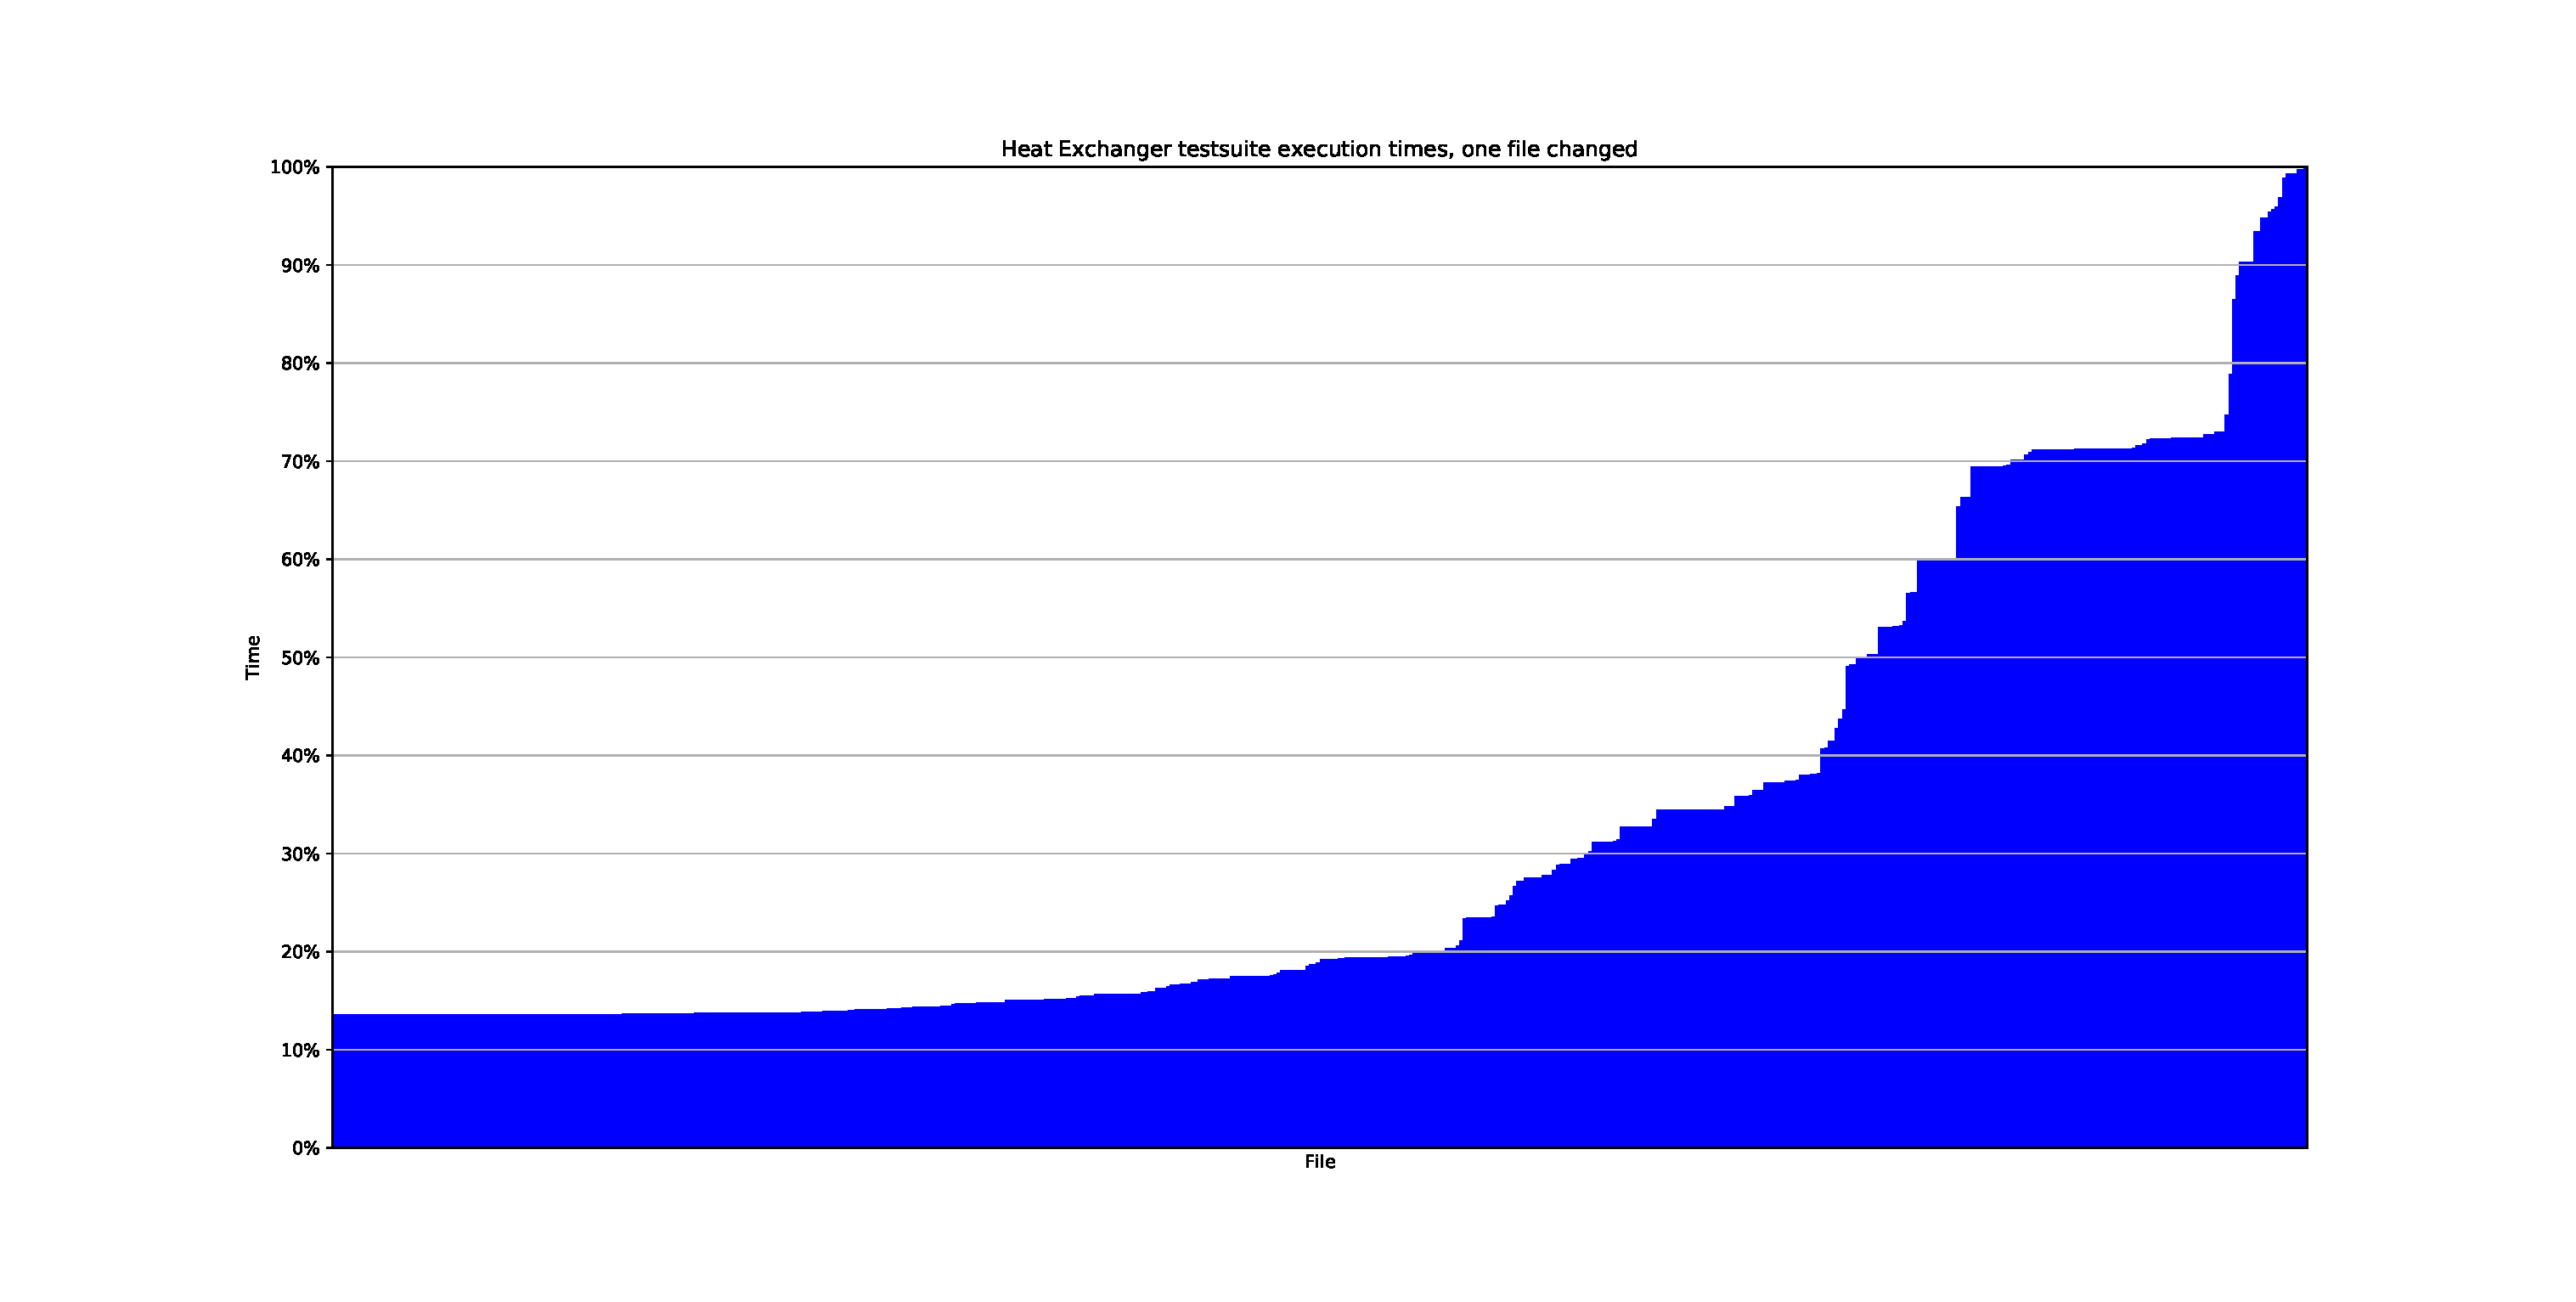
\includegraphics[width=\textwidth]{Graphs/HXL_one_file.eps}
    \caption{One file changed in HXL, 552 files in total. Average saving is 68 \%.}
    \label{fig:hxlonefile}
\end{figure}

\begin{figure}[!htbp]
    \centering
    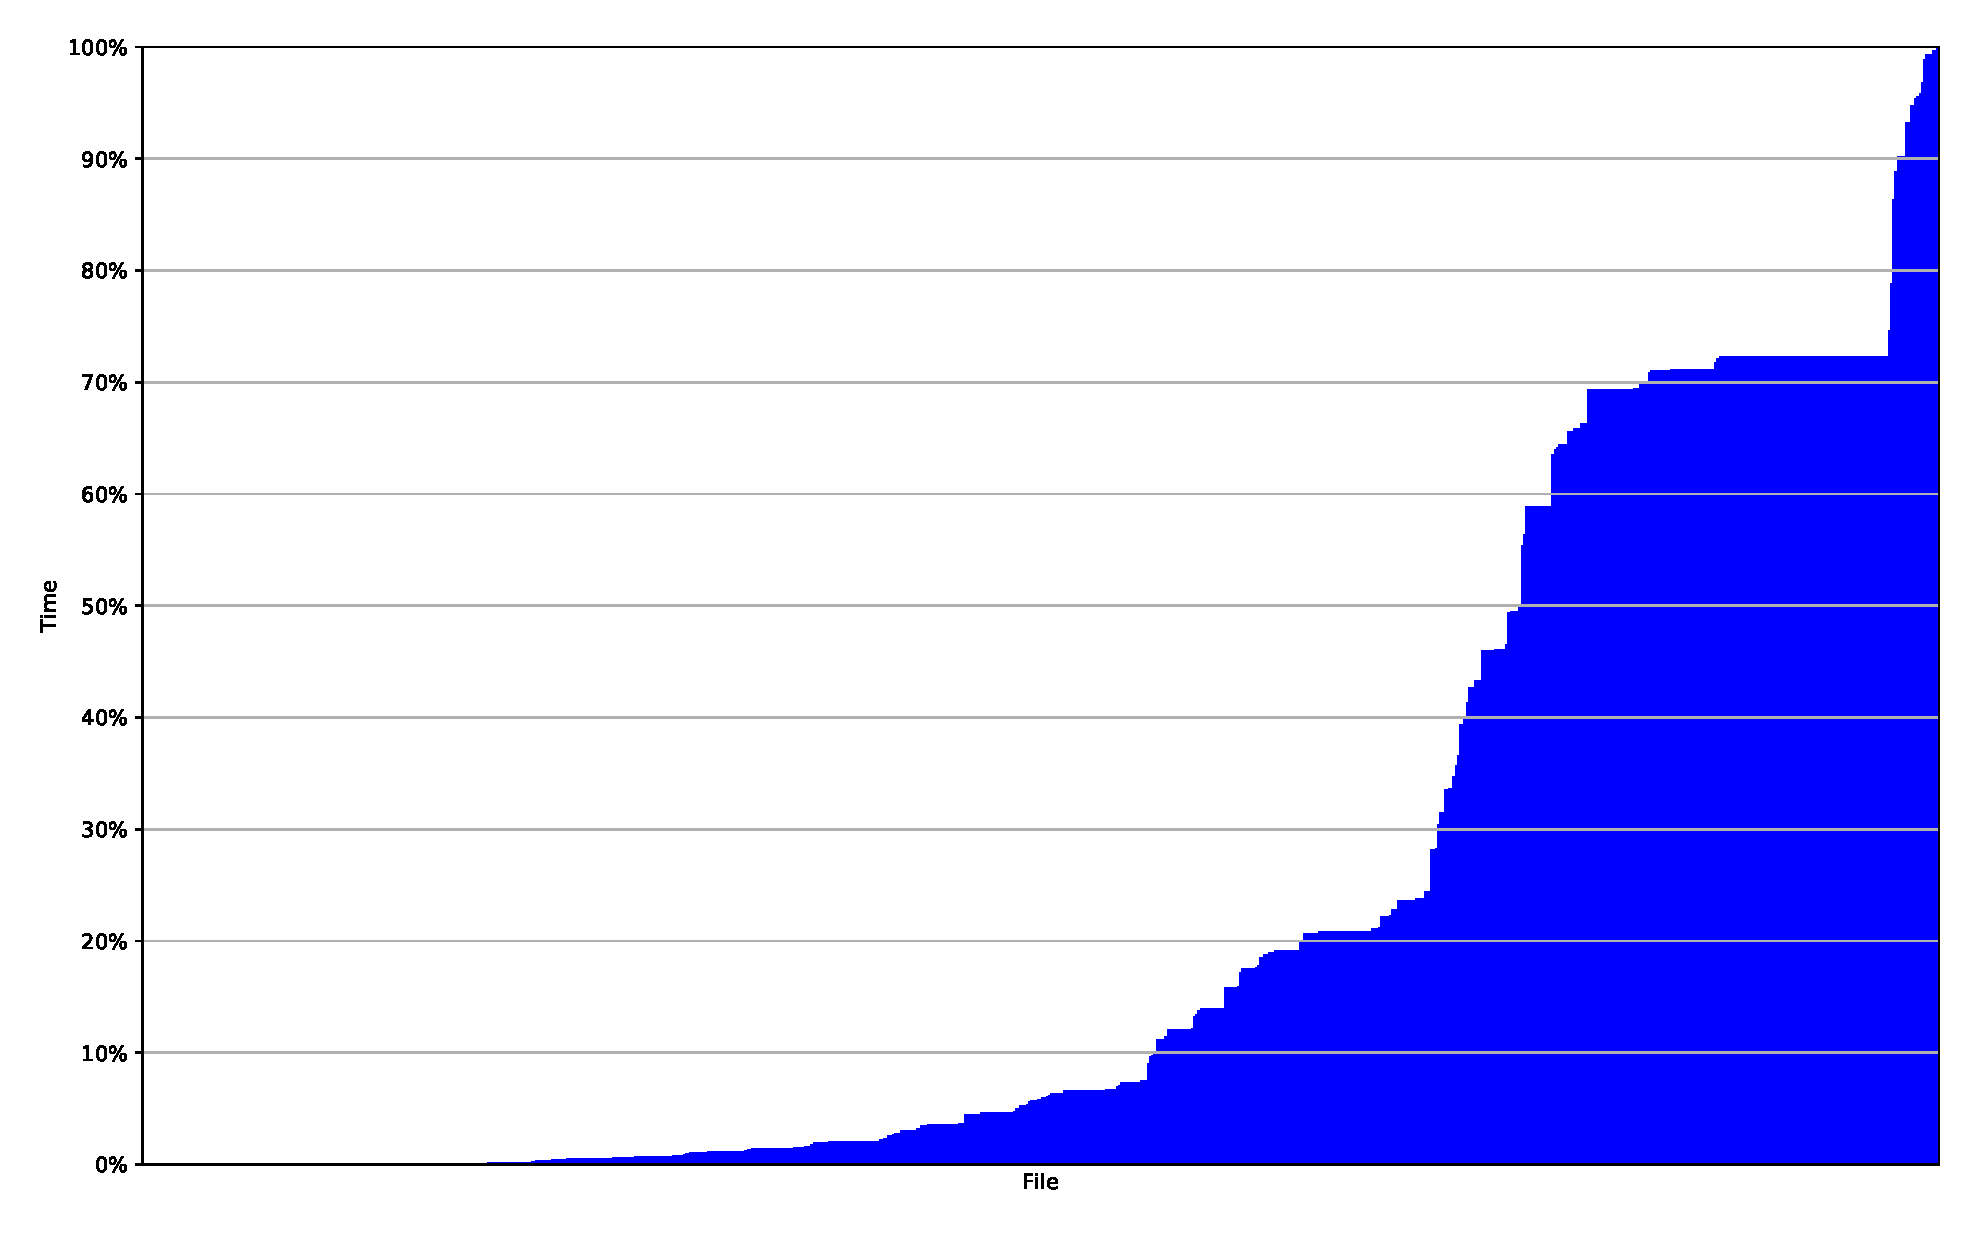
\includegraphics[width=\textwidth]{Graphs/HXL_one_model.eps}
    \caption{One class changed in HXL, 819 classes total. Average saving is 67 \%.}
    \label{fig:hxlonemodel}
\end{figure}

\begin{figure}[!htbp]
    \centering
    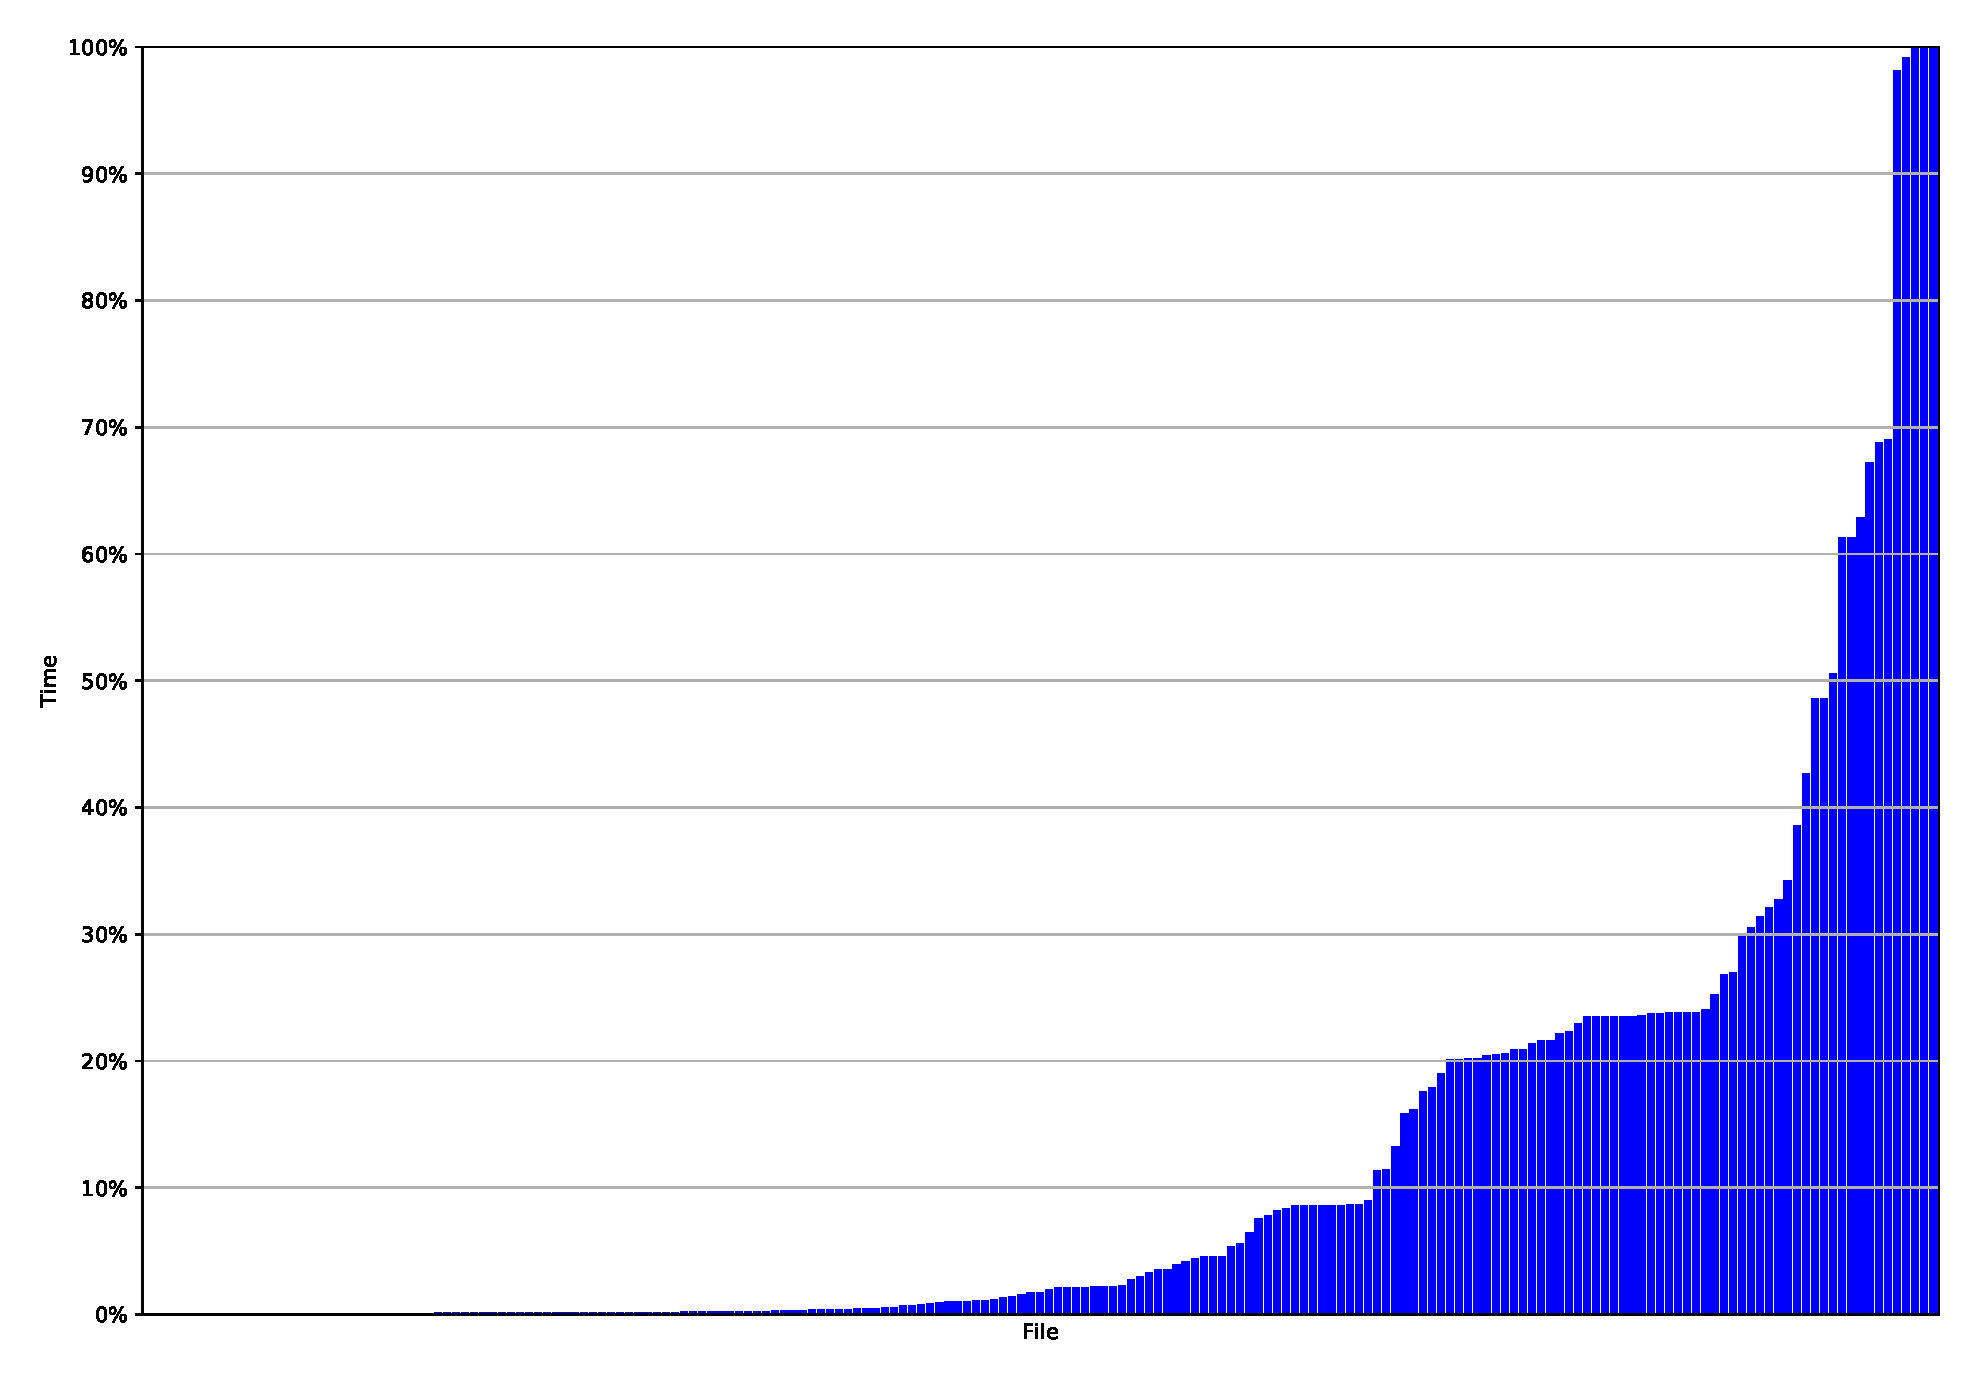
\includegraphics[width=\textwidth]{Graphs/MSL_one_file.eps}
    \caption{One file changed in MSL, 197 files in total. Average saving is 88 \%.}
    \label{fig:mslonefile}
\end{figure}

\begin{figure}[!htbp]
    \centering
    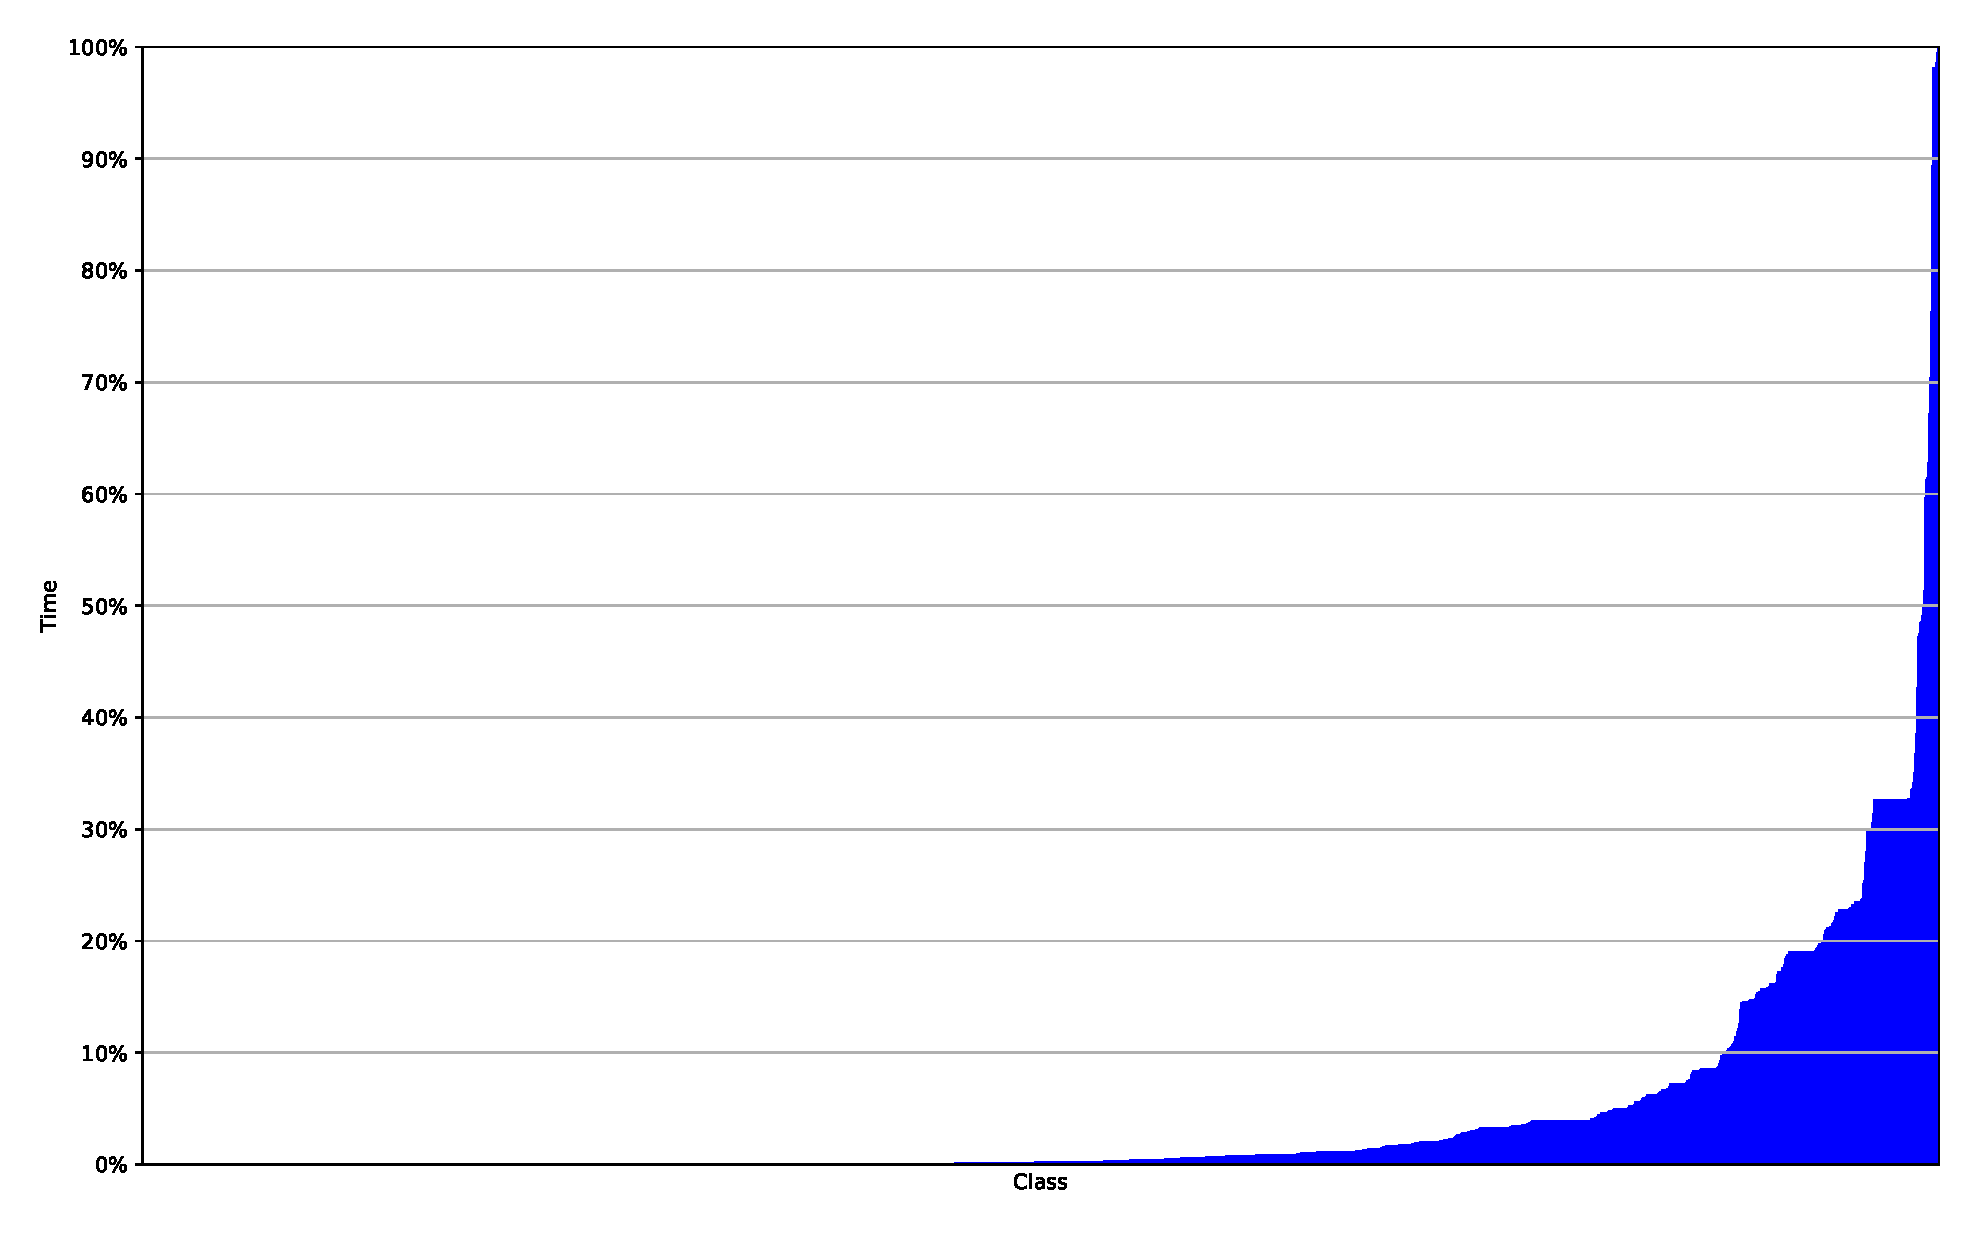
\includegraphics[width=\textwidth]{Graphs/MSL_one_model.eps}
    \caption{One class changed in MSL, 5917 classes total. Average saving is 93 \%. }
    \label{fig:mslonemodel}
\end{figure}

So far the results looks very good but they do not necessary reflect a real use case. In Figure \ref{fig:mslhistory} are all the commits in the commit history for MSL until commit e69f57, 24th of may 2017. On the y-axis we have commits and on the x-axis is the time for running the test selection corresponding to the commit. The time is plotted relative to the total time of the complete test suite. As the previous graphs the time for the dependency analysis is not included. Furthermore, we have not run the dependency analysis and test suite for each commit, instead the same dependency analysis and test suit results was reused for all commits. Running all tests and creating a new dependency analysis for every commit would require too much time. This means that the graph is an approximation. The average time saving for test executions in Figure \ref{fig:mslhistory} is 56\% (dependency analysis execution time excluded).

\begin{figure}[!htbp]
    \centering
    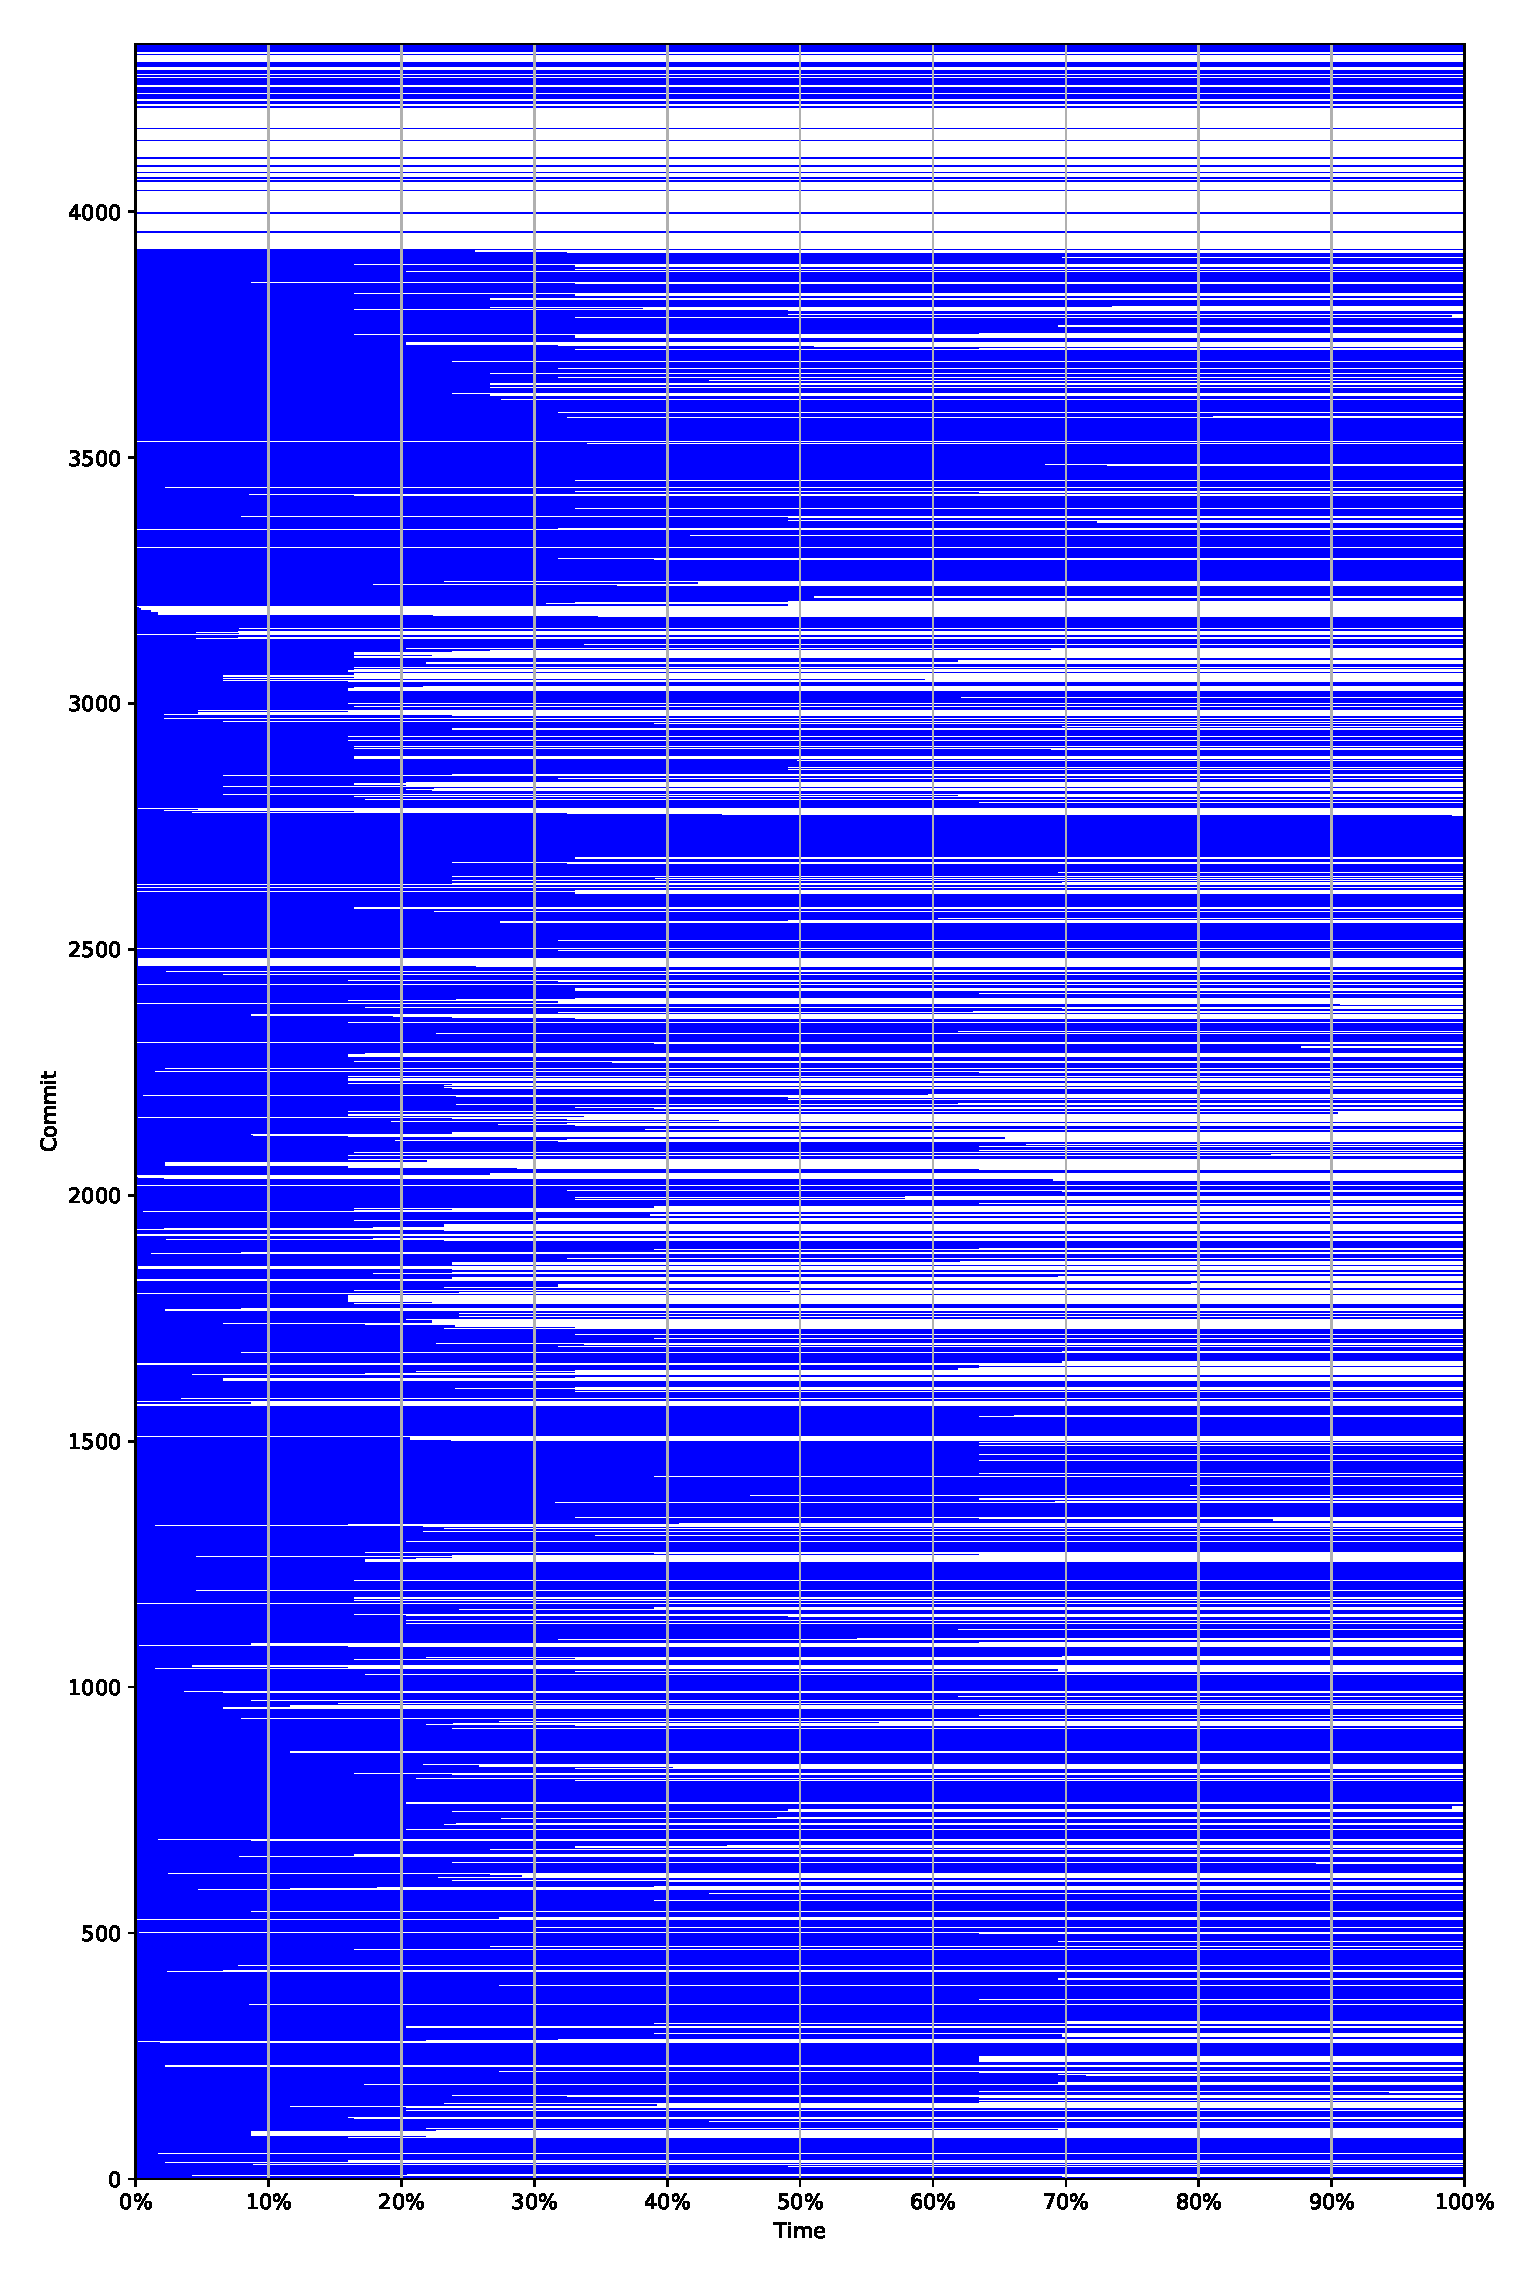
\includegraphics[width=\textwidth]{Graphs/MSL_history_plot.eps}
    \caption{History plot for 4341 commits from MSL. The average saving is 56 \%.}
    \label{fig:mslhistory}
\end{figure}

A breakdown of the graphs is shown in Table \ref{table:breakdown}, as well as some other information about the graphs. The \textit{Savings} are the average savings for each graph relative to the running time of the full test suite, found in the \textit{Complete test suite execution time} column. We also provide an average execution time for the dependency analysis. This was obtained by measuring the execution ten times, on the same computer used for the other results. However, it is usually not necessary to calculate the dependencies for all models or files unless every model or file is changed. Hence, the execution time is usually shorter in practice.

\begin{center}
\begin{table}[!htbp]
\begin{tabular}{|*{7}{c|}}
\cline{2-7}
      \multicolumn{1}{c|}{}
    & Figure
    & \multicolumn{2}{c|}{Units}
    & \makecell{Complete test suite \\ execution time}
    & \makecell{Dependency analysis \\ execution time}
    & Savings
\\ \hline
      \multirow{2}{*}{HXL}
    & \ref{fig:hxlonefile}
    & \multicolumn{1}{r}{552}
    & \multicolumn{1}{@{}l|}{files}
    & \multirow{2}{*}{3h 1m 51s}
    & \multirow{2}{*}{6.7s}
    &  68 \%
\\
    & \ref{fig:hxlonemodel}
    & \multicolumn{1}{r}{819}
    & \multicolumn{1}{@{}l|}{classes}
    &
    &
    & 67 \%
\\ \hline
      \multirow{3}{*}{MSL}
      & \ref{fig:mslonefile}
    & \multicolumn{1}{r}{197}
    & \multicolumn{1}{@{}l|}{files}
    & \multirow{3}{*}{2h 26m 35s}
    & \multirow{3}{*}{18.8s}
    & 88 \%
\\
    & \ref{fig:mslonemodel}
    & \multicolumn{1}{r}{5917}
    & \multicolumn{1}{@{}l|}{classes}
    &
    &
    & 93 \%
\\
    & \ref{fig:mslhistory}
    & \multicolumn{1}{r}{4341}
    & \multicolumn{1}{@{}l|}{commits}
    &
    &
    & 56 \%
    \\
\hline
\end{tabular}
\caption{Breakdown of Figure \ref{fig:hxlonefile} to \ref{fig:mslhistory} }
\label{table:breakdown}
\end{table}
\end{center}

\chapter[Discussion]{Discussion}
We have previously, in Chapter 3, discussed some aspects of the dependency analysis. We will now discuss a few other aspects of our work and then look at some related works.

\section{Validity}
Validating the test selection is an important step to make sure the test selection actually is safe. During the development of the dependency analysis we have developed a test suit which can validate that the dependency graph is correct for some Modelica libraries. However, is is not feasible to prove that the dependency analysis and our implementation is 100\% safe. Instead we have to try to prove that it is not safe, but that can never prove that what we have built is safe. But, it will increase our confidence for the test selection. 
%TODO: Rephrase, we do not hope to do
To do this we have a couple of approaches, firstly we hope to run our test selection parallel with the complete test suit on Modelon's build server to make sure all failed tests occurring have been caught by our test selection. This approach is inherently flawed since developers are actively trying to not commit code that breaks any tests.

Secondly we hope to do some mutation testing by introducing semi random errors in a library and then run all tests not in the test selection. If any test fails we know that the test selection is not safe. Both these approaches are essentially the same except mutation testing is probably more effective since we can guarantee that there is problems in the code base. However, depending on the test coverage, every test could still pass.

\section{Granularity}
%TODO: "Generally a more coarse analysis will have lower precision since classes in the same file will be considered having the same dependencies", is this really true?
%TODO: Write something about HXL where we get a better result for files than classes?
A dependency analysis can be performed with different granularities. Our dependency analysis handles classes and is sometimes converted to a more coarse analysis handling files. Generally a more coarse analysis will have lower precision since classes in the same file will be considered having the same dependencies. On the other hand moving to a more granular analysis can be costly ~\cite{DBLP:conf/sigsoft/LegunsenHSLZM16}, both in running time, complexity and size. A more granular analysis could for example handle dependencies between lines of code instead of classes. This would have to be weighted against the precision gained.

We chose class granularity because is was easy to implement. Initially we wanted to perform the analysis at file level but when we started implementing it it was natural to go to class level since all the class level dependencies had to be resolved anyway to find the corresponding files. The results shows significant saving and therefor it is not motivated to increase the precision at the cost of analysis complexity, development time and running time.

\section{Related Work}
% Kan kanske flyttas till bakgrunden ev till test selection delen. Måste inte ligga så sent i rapporten
A master thesis similar to this one has previously been done at LTH. In the previously master thesis JastAdd was used to decrease the cost for testing of Android projects ~\cite{kampe2012dependroid}. There is research done on test selection. A method for safe RTS for Java has been developed before, that has many similarities with the method we are developing for Modelica. 

Studies have been conducted to investigate at which granularity dependency analysis pays off the most and how much precision it can have without getting to expensive ~\cite{DBLP:conf/sigsoft/LegunsenHSLZM16}. It has also been done work in other techniques to achieve shorter time for testing, including dynamic test selection.

Safe regression test selection has been developed for Java at LTH \cite{DBLP:conf/pppj/OqvistHM16}. In this work the dependency graph is stored and updated when it changes unlike our solution for Modelica, where we compute the dependency graph each time. There is two main differences between Java and Modelica interesting for test selection. Modelica regression tests takes usually much longer time to run than Java regression tests. The longest time it takes to run all tests for a Java project used in the evaluation in \cite{DBLP:conf/pppj/OqvistHM16} is less than 20 seconds (on a 4-core 3.6GHz Intel i7-3820 CPU, with 64 GiB RAM, running Linux Mint 17.0). For the Modelica Standard Library it takes more than 2 hours to run all tests (on a Intel Core i5-4300M), even though the tests taking more than ten minutes, are canceled after ten minutes. In Modelica it is possible to use classes in another package without using imports, that is not possible in Java. This affects the dependency analysis.

\chapter[Conclusion]{Conclusion}
Our results show significant time savings when using test selection for Modelica projects. This was the one of the main goals of this thesis project. The other goal was to not compromise the testing quality when reducing the test suit. We have not proven that this is achieved but are confident that it is. 

\section{Future work}
We have succeeded in reducing the time for regression tests, but there is more work that can be done. Our test selection could be further evaluated. The same measurements we have performed for the commit history of the Modelica Standard Library could be performed for other Modelica libraries, to get a better understanding of how much time can be saved. The Modelica Standard Library is a git repository. For the libraries developed by Modelon, SVN is used. We have not had time to adopt our evaluation method to SVN.

Another thing that would be interesting to do, is to validate our test selection more. Like we mentioned in chapter 6 this could be done by running our test selection parallel with running the complete test suite on the build server and see if our test selection selects all tests that fails. Another option that might be better for validation is to use mutation testing and see if our test selection then selects all tests that fails.

It is possible that more time can be saved. It could be interesting to do the dependency analysis between lines of code instead of Modelica classes to see if that would save more time.

It would also be interesting to run the dependency analysis in the instance tree to see if the increased precision can save more time. But if all classes in a Modelica library should be instantiated in the instance tree, it will in the most cases require to much memory. So first a technique for throwing away parts of the instance tree along the process or some other solution must be developed. Doing this and running the dependency analysis in the instance tree will take more time than running the dependency analysis in the source tree. So the timed saved by a higher precision will have to be grater than the time lost by doing the dependency analysis in the instance tree.

\printbibliography[heading=bibintoc]

%\begin{appendices}
%\chapter{About This Document}
%\end{appendices}


\end{document}